\chapter{Property Graph Storage}
\label{sec:architecture:property}

The previous chapter described how \project{} stores and retrieves the structural graph: vertices, edges, and their topological relationships.
This chapter addresses the complementary problem of storing \emph{properties} and \emph{labels}.
A vertex's label determines its schema (e.g., Person vs.\ Post), and the properties are the attribute values attached to each vertex or edge under that schema.
\project{} introduces a bit-encoded label scheme that makes label extraction a single shift, and it offers two property storage modes, \emph{embedded} and \emph{columnar}, each suited to different access patterns.
A uniform property cursor abstraction lets query code switch between modes without modification.

%%%%%%%%%%%%%%%%%%%%%%%%%%%%%%%%%%%%%%%%%%%%%%%%%%%%%%%%%%%%%%%%%%%%%%%%%%%%%%%%
\section{Why Property Storage Is a Separate Problem}
\label{arch:prop-motivation}

Structural storage optimizes for topology traversal: sequential access to neighborhoods, fast degree lookups, and parallel scans across the vertex ID space.
Property storage optimizes for attribute access: point lookups on a single vertex's attributes, selective reads of one column across many vertices, and schema-aware type extraction.
These two access patterns demand different physical layouts.

Consider the LDBC Social Network Benchmark (SNB)~\cite{erling2015ldbc} Person vertex as a running example.
A PageRank computation iterates over every vertex's in-neighborhood and accumulates scores; it never reads \texttt{firstName}, \texttt{birthday}, or \texttt{browserUsed}.
A ``find person by name'' query reads string attributes for a single vertex; it never traverses edges.
If the database stores properties inline with the structural data, the PageRank scan loads property bytes it will never examine, wasting cache space and I/O bandwidth.
If the database stores properties in a separate table, the name-lookup query must issue an additional I/O to reach them after locating the vertex structurally.

Co-locating properties with structural data also creates write amplification.
In the EdgeKey representation (\autoref{sec:architecture:structural}), each vertex's sentinel row stores its in-degree and out-degree.
Appending a property blob to that sentinel means that every edge insertion (which updates the degree pair) must rewrite the entire sentinel row, including the property bytes that did not change.
Separating properties into their own tables eliminates this overhead but adds one cursor seek per hop for queries that need both structure and attributes.

This tension motivates offering both an embedded mode (properties co-located with structure) and a columnar mode (properties in separate per-label tables with column-group isolation).

\begin{figure}[t]
  \centering
  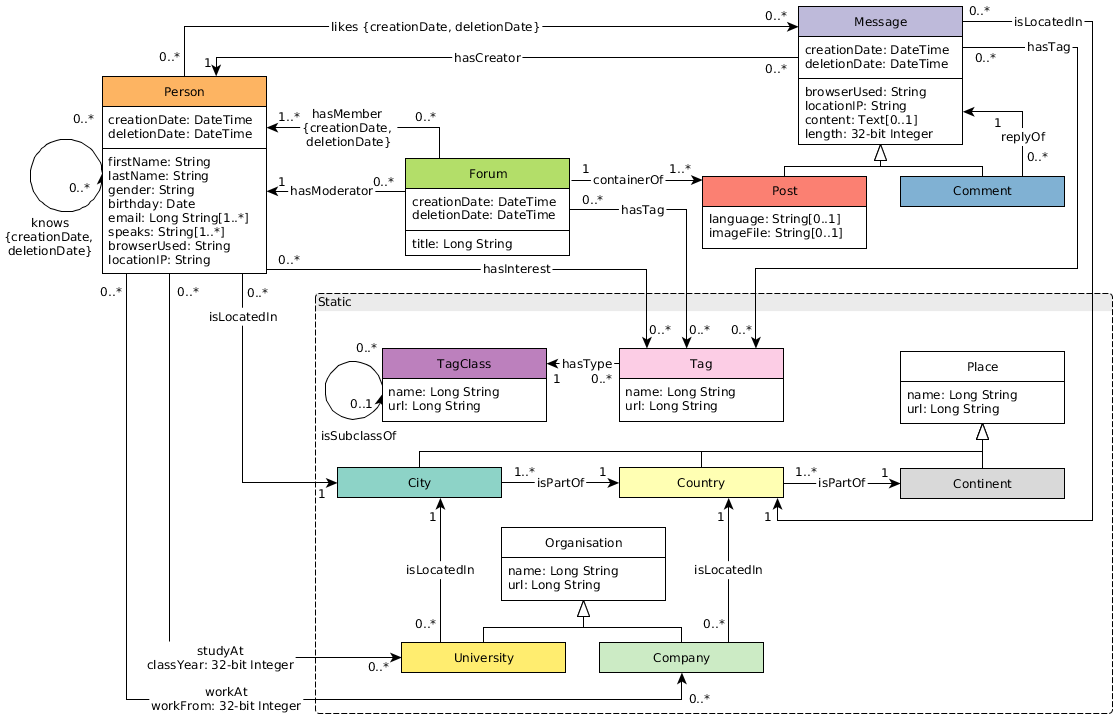
\includegraphics[width=\textwidth]{fig/schema.png}
  \caption{LDBC Social Network Benchmark schema~\cite[Figure 3.1]{angles2024ldbcsocialnetworkbenchmark}. Vertex types carry typed property fields; edge types connect specific endpoint pairs and may carry their own properties.}
  \label{fig:ldbc-snb-schema}
\end{figure}

\autoref{fig:ldbc-snb-schema} shows the LDBC SNB schema that serves as the running example throughout this chapter.
Two features of this schema surface design problems that a property storage layer must solve.
First, vertex types are independently numbered: a Person and a Post may share the same source ID, so the storage layer must disambiguate them.
Second, each pair of endpoint labels maps to exactly one edge type (\textsc{knows} connects only Person$\to$Person, \textsc{hasCreator} connects only Post$\to$Person), so edge labels can be inferred from endpoint labels without an explicit label column.

Both storage modes require knowing which schema applies to a given vertex, so we begin with label encoding before describing either mode.
The remainder of this chapter addresses four design questions:
\begin{enumerate}
  \item How to identify each vertex's label efficiently.
  \item How to store vertex and edge properties (inline vs.\ columnar).
  \item How to handle non-unique vertex IDs across labels.
  \item How to handle multi-valued attributes (e.g., a set of email addresses).
\end{enumerate}

%%%%%%%%%%%%%%%%%%%%%%%%%%%%%%%%%%%%%%%%%%%%%%%%%%%%%%%%%%%%%%%%%%%%%%%%%%%%%%%%
\section{Label Encoding}
\label{arch:label-encoding}

Labels assign vertices a type, and we use the terms interchangeably.
Vertices with the same label share an attribute schema (\autoref{sec:bg:model}): a \texttt{Person} vertex has \texttt{firstName}, \texttt{birthday}, and \texttt{email} columns, while a \texttt{Post} vertex has \texttt{content}, \texttt{creationDate}, and \texttt{length}.
The database must therefore identify each vertex's label so it can apply the correct schema, and it must do so without a table lookup on every access.

\subsection{Design Alternatives}
\label{arch:label-alternatives}

We considered three approaches before arriving at the labeled-vertex-ID scheme described in \autoref{arch:typed-ids}.
Each alternative's weakness motivates the next.
We illustrate the tradeoffs using LDBC SNB vertex types (Person, Post, Comment) and edge types (\texttt{knows}, \texttt{hasCreator}, \texttt{likes}).

\paragraph{Alternative 1: Duplicating representations.}
The simplest option maintains a separate graph representation per vertex label: one B-tree (or set of tables) for Person, another for Post, and so on.
Edges whose endpoints share a label stay within a single representation, so a \texttt{knows} edge between two Person vertices is straightforward.
However, an edge that crosses label boundaries, such as a \texttt{hasCreator} edge from a Post to a Person, spans two representations.
Traversing that edge requires a lookup into the destination label's table, an operation that is difficult to batch and that breaks sequential scan patterns.
\autoref{fig:label:two-reps} illustrates the problem: iterating through the neighborhood of a Post vertex in the Post table requires repeated random lookups into the Person table to resolve each \texttt{hasCreator} destination.

\begin{figure}[htbp]
  \centering
  
\includegraphics[width=0.7\textwidth]{two_reps.pdf}
  \caption{Duplicating representations: iterating the neighborhood of a source vertex requires cross-table lookups when edges span label boundaries.}
  \label{fig:label:two-reps}
\end{figure}

\paragraph{Alternative 2: Embedding a type attribute.}
To avoid maintaining multiple representations, a second option stores all vertices in a single graph and adds a ``source-type/destination-type'' attribute to each edge (or, equivalently, a ``type'' column in the edge table).
This eliminates cross-table joins, but filtering a vertex's neighborhood by destination type now requires scanning the entire neighborhood and checking the type attribute on each entry, because edges of different types are interleaved in the B-tree.
The scan is no longer sequential with respect to a single edge type.
\autoref{fig:label:embed-type} shows how both the EdgeKey and Adjacency List representations suffer from non-sequential access when the type attribute is embedded.

\begin{figure}[htbp]
  \centering
  \begin{subfigure}[b]{0.25\textwidth}
    \centering
    
\includegraphics[width=\linewidth]{relational_scenario_2a.pdf}
    \caption{EdgeKey}
    \label{fig:label:embed-type:ekey}
  \end{subfigure}
  \hfill
  \begin{subfigure}[b]{0.70\textwidth}
    \centering
    
\includegraphics[width=\linewidth]{relational_scenario_2b.pdf}
    \caption{Adjacency List}
    \label{fig:label:embed-type:adjlist}
  \end{subfigure}
  \caption{Embedding a type attribute eliminates cross-table lookups but creates non-sequential access: filtering by destination type requires scanning all entries and checking the type column.}
  \label{fig:label:embed-type}
\end{figure}

\paragraph{Alternative 3: Vertex re-labelling (ID-space partitioning).}
A third option partitions the vertex ID space by label.
All Person vertices receive IDs in one contiguous range, all Post vertices in another, and so on.
Because \wt{} stores keys in sorted order, all vertices of a given label are contiguous in the B-tree; a label-filtered scan is a simple key-range bound, and access within a label is sequential.

The drawback is that the range boundaries depend on vertex counts at load time: the system must decide up front how many IDs to reserve for each label.
If a label's allocation is exhausted, re-partitioning is expensive.
Our candidacy prototype implemented this approach as a user-space framework that re-mapped original vertex IDs into partitioned ranges and maintained a bidirectional mapping table.
\autoref{fig:label:relabel} illustrates the re-labelled ID space.

\begin{figure}[htbp]
  \centering
  
\includegraphics[width=\textwidth]{relational_scenario_3.pdf}
  \caption{Vertex re-labelling: partitioning the vertex ID space by label gives sequential access within a type but requires boundaries fixed at load time.}
  \label{fig:label:relabel}
\end{figure}

\subsection{Labeled Vertex IDs}
\label{arch:typed-ids}

\project{}'s labeled-vertex-ID scheme refines Alternative~3 (ID-space partitioning) by fixing the partition boundaries at schema definition time rather than at load time.
\project{} reserves the top 8 bits of the 64-bit vertex ID as a \emph{label tag}; the remaining 56 bits hold a label-local counter:
\[
  \texttt{id} = \underbrace{L}_{\text{8 bits}} \;\|\; \underbrace{\text{counter}}_{\text{56 bits}}
\]
Extracting the label is a single shift, and the range of all vertices with label~$L$ is a static interval; neither requires runtime state:
\[
  \textsc{vtype\_of}(\texttt{id}) = \texttt{id} \gg 56
  \qquad
  \text{range}(L) = \bigl[L \ll 56,\; (L{+}1) \ll 56\bigr)
\]

Because \wt{} sorts keys lexicographically via \texttt{memcmp}, all IDs are stored as big-endian 8-byte blobs: big-endian layout makes byte order coincide with numeric order, and raw comparison avoids the decoding overhead of \wt{}'s native variable-length integer formats (\texttt{I}, \texttt{Q}).
After this byte-swap, the label tag occupies the first byte of the stored key, so \wt{}'s lexicographic comparison groups vertices with the same label contiguously in the B-tree.
A label-filtered scan is therefore a simple key-range bound.

Edge labels are determined implicitly from the labels of their endpoints.
We assume that each pair of endpoint labels maps to exactly one edge label, a condition that holds in the LDBC SNB schema (\autoref{fig:ldbc-snb-schema}).
Under this assumption, no label column is needed in the edge key, and the edge label is recovered by inspecting \code{VTYPE\_OF(src)} and \code{VTYPE\_OF(dst)}.

This design contrasts with two alternatives.
TuGraph~\cite{linBuildingHighPerformanceGraph2024} stores the label in the vertex \emph{value}, requiring a value read to determine it.
GraphflowDB~\cite{graphflowdb2021Gupta} assigns consecutive ID ranges per label, but the range boundaries depend on the actual vertex counts at load time.
\project{}'s bit-reservation gives $O(1)$ label extraction with boundaries that are fixed at schema definition time.

%%%%%%%%%%%%%%%%%%%%%%%%%%%%%%%%%%%%%%%%%%%%%%%%%%%%%%%%%%%%%%%%%%%%%%%%%%%%%%%%
\section{Embedded Mode}
\label{arch:prop-embedded}

In embedded mode, properties are stored as an opaque byte blob alongside the structural data.
The schema for each label is defined as a packed C struct.
For example, the LDBC SNB Person schema is a 153-byte struct containing fields for \texttt{creationDate} (8\,B), \texttt{birthday} (8\,B), \texttt{firstName} (40\,B), \texttt{lastName} (40\,B), \texttt{gender} (8\,B), \texttt{browserUsed} (25\,B), and \texttt{locationIP} (24\,B).
Writing a vertex's properties is a \code{memcpy} of the struct into a \wt{} \code{WT\_ITEM}; reading is a pointer cast back to the struct type, a zero-copy, zero-deserialization operation.

For the EdgeKey representation, vertex properties are appended after the degree bytes in the sentinel entry: the value of a vertex entry becomes \texttt{[in\_degree\,|\,out\_degree\,|\,property\_blob]}.
Edge properties are stored in the edge row's value field.
Reading a vertex's properties and degree thus requires a single cursor lookup.

The Adjacency List representation cannot embed properties in the same way, because the \code{value\_format=u} required by \code{WT\_MODIFY} (\autoref{arch:adjlist}) precludes typed columns in the adjacency table's value.
AdjList instead uses a scheme similar to TuGraph's: properties go into separate \code{node\_props} and \code{edge\_props} tables, keyed by the same IDs, with the schema determined by \code{VTYPE\_OF(id)}.

The embedded layout incurs a write-amplification cost in the EdgeKey representation: every edge insertion that updates a vertex's degree must rewrite the full sentinel row, including the appended property blob.
For the Person label with its 153-byte schema, each degree update rewrites at least 161 bytes (8 bytes of degrees plus 153 bytes of properties), even though only 8 bytes (the degree pair) changed.

\begin{figure}[htbp]
  \centering
  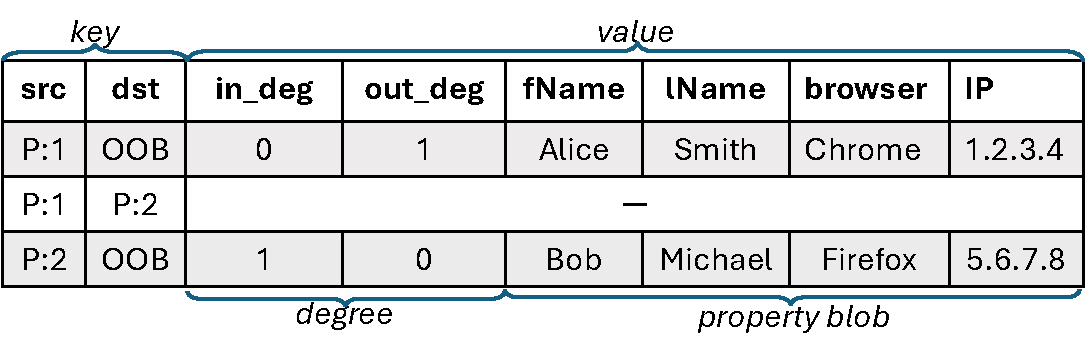
\includegraphics[width=0.75\textwidth]{fig/ekey_embedded_schema.pdf}
  \caption{Embedded property storage for Person vertices (EdgeKey).
    All properties are packed into the sentinel row's value alongside the degree pair; every read fetches the full record.}
  \label{fig:schema:property:embedded}
\end{figure}

%%%%%%%%%%%%%%%%%%%%%%%%%%%%%%%%%%%%%%%%%%%%%%%%%%%%%%%%%%%%%%%%%%%%%%%%%%%%%%%%
\section{Columnar Mode}
\label{arch:prop-columnar}

In columnar mode, properties are stored in separate \emph{per-label} tables with \wt{} column groups.
Each vertex label gets its own property table (e.g., \code{person\_props}, \code{post\_props}), and each edge label with properties gets a dedicated table (e.g., \code{knows\_props}, \code{likes\_props}).

\paragraph{Column groups in \wt{}.}
A \wt{} column group physically splits a table's value columns into a separate B-tree.
When a table has multiple column groups, each group's data lives in its own B-tree file; a cursor opened on one column group reads only that group's pages (e.g., \code{colgroup:person\_props:temporal} reads only that temporal column).
Omitting a \code{get\_value()} call on a column group is not sufficient to avoid I/O: \wt{} loads entire pages into its buffer pool regardless of whether the application reads the value.
Column groups fix this by placing different columns in physically separate B-trees, so pages from one group are never loaded during a scan that targets a different group.

\paragraph{Column-group assignments.}
We \textbf{separate fixed-size, scan-friendly columns from variable-length ones}: fixed-size groups yield high row density per page, while isolating variable-length columns keeps large blobs out of the buffer pool during narrow scans.

For the LDBC SNB schema, we assign column groups as follows:
\begin{itemize}
  \item \textbf{Person:}
    \code{temporal} --- \texttt{creationDate}, \texttt{birthday} (16\,B/row, fixed-size);
    \code{name} --- \texttt{firstName}, \texttt{lastName}, \texttt{gender} (variable-size);
    \code{contact} --- \texttt{browserUsed}, \texttt{locationIP} (variable-size).
  \item \textbf{Post:}
    \code{temporal} --- \texttt{creationDate}, \texttt{length} (12\,B/row, fixed-size);
    \code{meta} --- \texttt{browserUsed}, \texttt{locationIP}, \texttt{language}, \texttt{imageFile} (variable-size);
    \code{content} --- \texttt{content} (isolated because it can be up to 2{,}000 characters, and mixing it with compact metadata columns would destroy row density).
  \item \textbf{Comment:} structured similarly to Post, with \code{temporal}, \code{meta}, and \code{content} groups.
\end{itemize}

An analytical query that filters Person vertices by creation date scans only the \code{temporal} B-tree, reading 16 bytes per row instead of the full 153-byte property record.

\paragraph{Interaction with structural representations.}
Both structural representations use the same per-label property tables in columnar mode.
For AdjList, this replaces untyped blob tables with typed column-group tables.
For EdgeKey, the sentinel row shrinks to 8 bytes (degrees only), keeping the structural B-tree compact.
Contrast \autoref{fig:schema:property:embedded} with \autoref{fig:schema:property:columnar}.

\begin{figure}[htbp]
  \centering
  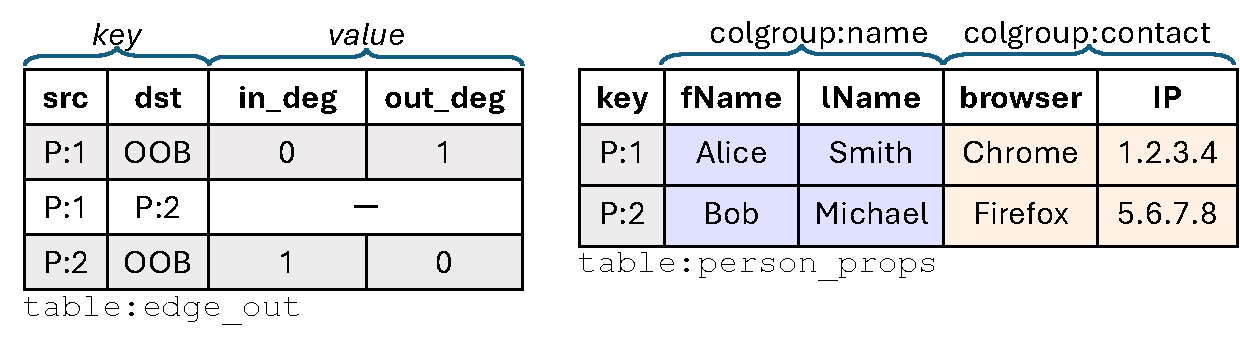
\includegraphics[width=0.85\textwidth]{fig/ekey_col_schema.pdf}
  \caption{Columnar property storage for Person vertices (EdgeKey).
    Sentinel rows store only degrees (8\,B); properties are split into per-label column-group B-trees, so scanning one attribute reads only that group's pages.}
  \label{fig:schema:property:columnar}
\end{figure}

To our knowledge, \project{} is the first system to provide \textbf{disk-based columnar property access on a graph storage engine}; per-column I/O isolation inherits \wt{}'s ACID transactions, MVCC, crash recovery, and buffer pool management without re-implementation.
GraphflowDB~\cite{graphflowdb2021Gupta} achieves columnar access but operates entirely in memory; TuGraph~\cite{linBuildingHighPerformanceGraph2024} is disk-based but packs all properties into a single blob with no per-column isolation.

\paragraph{Multi-valued attributes.}
Multi-valued attributes (e.g., a Person's set of email addresses) cannot be stored in typed columns because the number of values per vertex varies.
These are handled by secondary tables with composite keys \texttt{(vertex\_id, index)}, storing one value per row, retrieved via a prefix range scan on the vertex's ID.

%%%%%%%%%%%%%%%%%%%%%%%%%%%%%%%%%%%%%%%%%%%%%%%%%%%%%%%%%%%%%%%%%%%%%%%%%%%%%%%%
\section{Choosing Between Modes}
\label{arch:prop-choosing}

The embedded and columnar modes represent different points in a performance tradeoff space.
This section provides a qualitative comparison; we quantify the tradeoff experimentally in \autoref{sec:eval:emb-vs-col}.

\paragraph{Point queries.}
For a single-vertex property lookup, both modes require one cursor seek: embedded mode seeks into the structural table and reads the property blob from the sentinel row (EdgeKey) or the \code{node\_props} table (AdjList); columnar mode seeks into the per-label property table.
Performance is similar.

\paragraph{Multi-hop traversals with property access.}
Embedded mode has an advantage when a query traverses multiple hops and reads properties at each hop.
In EdgeKey's embedded mode, each hop's structural lookup already delivers the destination vertex's properties in the same sentinel row (one I/O per hop).
In columnar mode, each hop requires an additional seek into the destination's property table (two I/Os per hop).

\paragraph{Analytical scans filtering by a single attribute.}
Columnar mode excels when a query scans many vertices but reads only one or two columns.
The query opens a cursor on the relevant column group's B-tree and reads only that group's pages.
In embedded mode, the same scan reads full property records, loading columns it will not examine.

\paragraph{Per-label deployment.}
The choice between modes can be made per-label based on the expected workload.
A label accessed primarily by analytical scans (e.g., Post, where a BI query filters by creation date) benefits from columnar storage.
A label accessed primarily by multi-hop traversals with property filters (e.g., Person in a friend-of-friend search that checks age) benefits from embedded storage.

%%%%%%%%%%%%%%%%%%%%%%%%%%%%%%%%%%%%%%%%%%%%%%%%%%%%%%%%%%%%%%%%%%%%%%%%%%%%%%%%
\section{Property Cursors}
\label{arch:prop-cursors}

The two storage modes require different \wt{} operations to read properties: columnar mode opens a column-group cursor and advances through a single B-tree; embedded mode extracts fields from an opaque byte blob using schema-specific offsets.
\project{} hides this difference behind a uniform cursor abstraction so that query code is mode-agnostic.

\subsection{Abstract Interface}
\label{arch:prop-cursors:interface}

Two abstract base classes define the property cursor \ac{API}: \code{NodePropCursor} for vertex properties and \code{EdgePropCursor} for edge properties.

\code{NodePropCursor} supports two positioning modes: \code{set\_range(start, end)} for sequential scans across a vertex ID range, and \code{seek(id)} for point lookups on a single vertex.
After positioning, \code{next()} advances to the next vertex, and typed accessors (\code{get\_uint64(n)}, \code{get\_int32(n)}, \code{get\_string(n)}) extract individual columns by index.

\code{EdgePropCursor} supports \code{set\_src(src)} to pin a source vertex and iterate over its outgoing edges' properties, and \code{set\_src\_range(start, end)} for bulk scans.
It provides the same typed accessors as \code{NodePropCursor}.

\autoref{tab:propapi} summarizes the property \ac{API}.
The first group lists \code{GraphBase} methods for raw property access and cursor creation; the remaining groups list the abstract cursor interfaces.

\begin{table}[ht!]
\centering
  \small
  \begin{tabularx}{\textwidth}{|>{\hsize=\dimexpr 0.35\hsize+0.1\tabcolsep+0.2\arrayrulewidth\relax}X
    |>{\hsize=\dimexpr 0.65\hsize-0.1\tabcolsep-0.2\arrayrulewidth\relax}X|}
  \hline
  \rowcolor[HTML]{FFE135}
  \textbf{Operation}        &\textbf{Interface}                                       \\ \hline
  Set vertex properties     &\apicall{void set_node_properties(node_id_t id, const uint8_t* data, size_t size)}  \\ \hline
  Get vertex properties     &\apicall{prop_blob get_node_properties(node_id_t id)}    \\ \hline
  Set edge properties       &\apicall{void set_edge_properties(node_id_t src, node_id_t dst, const uint8_t* data, size_t size)}  \\ \hline
  Get edge properties       &\apicall{prop_blob get_edge_properties(node_id_t src, node_id_t dst)}  \\ \hline
  Create node property cursor &\apicall{NodePropCursor *get_node_prop_cursor(string table, string colgroup)}  \\ \hline
  Create edge property cursor &\apicall{EdgePropCursor *get_edge_prop_cursor(string table, string colgroup)}  \\ \hline
  \rowcolor[HTML]{FFE135}
  \textbf{NodePropCursor}   &\textbf{}                                                \\ \hline
  Set scan range            &\apicall{void set_range(node_id_t start, node_id_t end)} \\ \hline
  Point lookup              &\apicall{bool seek(node_id_t id)}                        \\ \hline
  Advance to next vertex    &\apicall{bool next()}                                    \\ \hline
  Current vertex ID         &\apicall{node_id_t key()}                                \\ \hline
  Read \code{uint64} column &\apicall{uint64_t get_uint64(int n)}                     \\ \hline
  Read \code{int32} column  &\apicall{int32_t get_int32(int n)}                       \\ \hline
  \rowcolor[HTML]{FFE135}
  \textbf{EdgePropCursor}   &\textbf{}                                                \\ \hline
  Pin source vertex         &\apicall{void set_src(node_id_t src)}                    \\ \hline
  Set source range          &\apicall{void set_src_range(node_id_t start, node_id_t end)}  \\ \hline
  Point lookup              &\apicall{bool seek(node_id_t src, node_id_t dst)}        \\ \hline
  Advance to next edge      &\apicall{bool next()}                                    \\ \hline
  Current source            &\apicall{node_id_t src()}                                \\ \hline
  Current destination       &\apicall{node_id_t dst()}                                \\ \hline
  Read \code{uint64} column &\apicall{uint64_t get_uint64(int n)}                     \\ \hline

  \end{tabularx}
\caption{Property \ac{API}.  The first group extends the \code{GraphBase} interface from \autoref{tab:graphapi} with property access and cursor factory methods.  \code{NodePropCursor} and \code{EdgePropCursor} are abstract base classes; columnar and embedded implementations are described in \autoref{arch:prop-cursors:columnar} and \autoref{arch:prop-cursors:embedded}.}
\label{tab:propapi}
\end{table}

\subsection{Columnar Implementation}
\label{arch:prop-cursors:columnar}

The columnar implementation (\code{WTNodePropCursor}, \code{WTEdgePropCursor}) wraps a raw \wt{} column-group cursor.
\code{set\_range()} positions the cursor via \code{search\_near()}, and \code{next()} advances the \wt{} cursor, reading only the column group's B-tree pages.

Each column group has a layout described by a \code{ColgroupValueLayout} enum (e.g., \code{CVL\_Q} for a single \code{uint64}, \code{CVL\_QQ} for two \code{uint64}s, \code{CVL\_Qi} for a \code{uint64} and an \code{int32}).
The layout determines the arity of the \code{get\_value()} call issued to \wt{}, avoiding unnecessary unpacking of columns in other groups.

\code{WTEdgePropCursor} includes a \code{node\_keyed} flag that adapts the cursor to single-key vertex-property tables.
This lets query code use a uniform edge-cursor interface even when reading vertex properties of a traversal's destination, simplifying multi-hop query implementations.

\subsection{Embedded Implementation}
\label{arch:prop-cursors:embedded}

The embedded implementation (\code{EmbNodePropCursor}, \code{EmbEdgePropCursor}) uses schema-specific extractor function pointers (\code{I64Extractor}, \code{I32Extractor}) to pull typed fields from opaque property blobs at compile-time-known byte offsets.

\code{EmbNodePropCursor} has two scan paths depending on the structural representation.
With EdgeKey, it opens a direct \wt{} cursor on the structural table and reads the property blob from the sentinel row's value suffix.
With AdjList, it opens a cursor on the \code{NODE\_PROPS\_TABLE} and iterates through it, since AdjList stores properties separately.

\code{EmbEdgePropCursor} pre-fetches the neighbor list for a source vertex via \code{get\_out\_nodes\_id()}, filters by destination vertex type using \code{VTYPE\_OF()}, and issues one \code{get\_edge\_properties()} call per matching neighbor.

\subsection{Factory Methods and Mode Transparency}
\label{arch:prop-cursors:factory}

\code{GraphBase} provides factory methods (\code{get\_node\_prop\_cursor()}, \code{get\_edge\_prop\_cursor()}) that select the concrete cursor implementation based on the storage mode configured for each label.
Query code calls \code{set\_range()}, \code{next()}, and \code{get\_uint64()} without knowing whether properties come from a column-group B-tree or an embedded blob.

This design mirrors the topology cursor abstraction described in \autoref{appendix:iterators}: just as \code{OutCursor} hides whether the underlying representation is AdjList or EdgeKey, \code{NodePropCursor} hides whether properties are stored in column groups or inline with the structure.
The full class hierarchy and annotated code listings appear in \autoref{chap:appendix:prop-cursors}.

%%%%%%%%%%%%%%%%%%%%%%%%%%%%%%%%%%%%%%%%%%%%%%%%%%%%%%%%%%%%%%%%%%%%%%%%%%%%%%%%
\section{Bulk Loading Properties}
\label{arch:prop-bulk-load}

Loading the full LDBC SNB dataset into \project{} requires coordinating property writes with edge insertions and managing RAM for ID translation across vertex types.
This section describes the property-aware bulk loader and explains how the storage decisions from the preceding sections constrain its pipeline.

\subsection{The Ordering Constraint}
\label{arch:prop-bulk:ordering}

In EdgeKey's embedded mode, a vertex's sentinel row stores both its degree pair and its property blob (\autoref{arch:prop-embedded}).
Each \code{add\_edge} call updates the degree pair; each \code{set\_node\_properties} call writes the full sentinel value, including the property blob.
If properties are written before all edges have been inserted, a subsequent \code{add\_edge} overwrites the sentinel and discards the property bytes.
Property writes must therefore follow all edge insertions.

Columnar mode does not have this constraint, because properties and degrees live in separate tables.
The loader preserves the stricter ordering regardless of mode so that the same pipeline works for both.

\subsection{Deferred Writes via Spool Files}
\label{arch:prop-bulk:spool}

The ordering constraint means vertex properties cannot be written during vertex loading.
Accumulating all property blobs in memory until the edge phase completes is expensive: at SF-10, the Comment type alone has approximately 15 million variable-length records.

The loader instead streams each property record to a binary spool file on disk.
A node-property record is \texttt{[typed\_id(8\,B)\,|\,size(4\,B)\,|\,data[]]};
an edge-property record adds source and destination fields: \texttt{[src(8\,B)\,|\,dst(8\,B)\,|\,size(4\,B)\,|\,data[]]}.
The flush phase reads each spool sequentially and issues one \code{set\_node\_properties} or \code{set\_edge\_properties} call per record, buffering only the current record.

\subsection{ID Translation}
\label{arch:prop-bulk:id-map}

LDBC SNB CSVs use plain integer IDs.
The loader translates each CSV ID into a labeled vertex ID (\autoref{arch:typed-ids}) via per-type \code{SnbIdMap}s: sorted vectors of \texttt{(ldbc\_id, typed\_id)} pairs supporting $O(\log n)$ binary-search lookup.
At 16 bytes per entry, these use less than half the memory of an equivalent \code{std::unordered\_map} (40--50 bytes per entry with bucket overhead).
At SF-10, the comment ID map drops from approximately 600\,MB to 240\,MB.
After the vertex phase, each map is read-only; concurrent lookups during edge loading require no synchronization.

\subsection{Pipeline Phases}
\label{arch:prop-bulk:phases}

The loader runs five phases.
Each thread creates its own \code{GraphBase} handle (and therefore its own \wt{} session), so there is no handle-level contention.

\paragraph{Phase~1: Vertex loading.}
All vertex types except Forum load in parallel, one thread per type.
Each thread reads its CSV, assigns labeled vertex IDs via \code{MAKE\_TYPED\_ID}, inserts vertices with zero initial degrees, and writes property blobs to a per-type spool file.
Forum vertices load sequentially afterward, because the Forum schema embeds the moderator's typed Person~ID, which requires the Person ID map.

\paragraph{Phase~2: Edge loading.}
Phase~2a loads all edges not involving Comment vertices in parallel.
Phase~2b loads Comment-touching edges one type at a time, with internal multi-threading within each type, to avoid write-write contention on high-degree Comment adjacency-list entries (\autoref{arch:prop-bulk:concurrency}).

Edges with properties (\texttt{knows}, \texttt{likes}, \texttt{hasMember}, \texttt{studyAt}, \texttt{workAt}) write their attribute bytes to edge-property spool files during this phase.

\paragraph{Phase~3: Flush vertex properties.}
Each vertex type's spool is replayed in parallel.
Person properties receive a patch: the \code{country\_id} field, derived by joining \texttt{person\_isLocatedIn\_place} and \texttt{place\_isPartOf\_place}, is resolved between Phase~2 and Phase~3 and written into the Person blob before it is committed.

\paragraph{Phase~4: Flush edge properties.}
Edge-property spools are replayed in parallel.
If an edge was lost to an unrecovered \code{WT\_ROLLBACK} during Phase~2, the flush phase re-inserts it before applying the property record.

\paragraph{Phase~5: Secondary tables.}
Multi-valued attributes (\code{person\_email}, \code{person\_speaks}) load from their CSVs directly into the secondary tables described in \autoref{arch:prop-columnar}.

\subsection{Concurrency and Conflict Handling}
\label{arch:prop-bulk:concurrency}

Parallel edge insertion creates write-write conflicts when two threads update the same vertex's degree counter within the same \wt{} snapshot transaction.
\wt{} detects this and returns \code{WT\_ROLLBACK}, aborting the transaction.
The loader retries each \code{add\_edge} up to 500 times; after a rollback, the retrying thread sees the winner's committed state and can proceed.

When Comment-touching edge types ran concurrently in early versions of the loader, threads competed on the same high-degree Comment entries, causing retry loops of up to 500 iterations per edge.
Serializing Comment edge types into Phase~2b eliminated this cross-type contention.
